\beginsong{Foggy dew}[
    wuw={Canon Charles O'Neill}, 
    jahr={1919},
    bo={322}, 
    pfii={186}, 
    gruen={290}, 
    siru={230}, 
    index={'Twas down the glen},
]

\beginverse 
\endverse
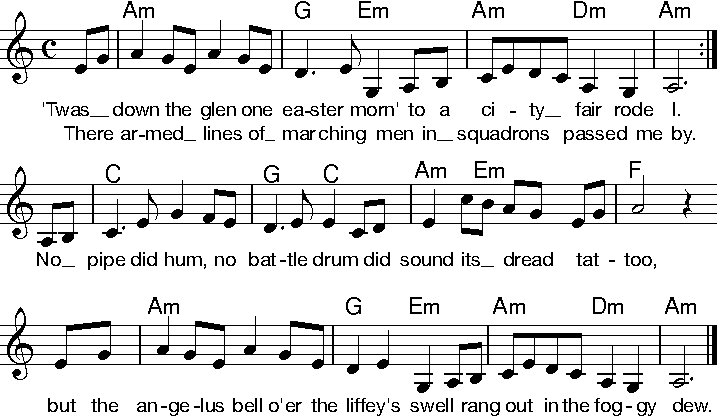
\includegraphics[draft=false, width=1\textwidth]{Noten/Lied045.pdf}	

\beginverse\memorize
'Twas Brit\[Am]tania bade our \[G]wild geese \[Em]go, that small \[Am]nations \[Dm]might be \[Am]free,
but their lonely graves are by \[G]Sulva's \[Em]waves or the \[Am]shore of the \[Dm]great North \[Am]Sea.
Oh, \[C]had they died by \[G]Peare's \[C]side or had \[Am]fought with \[Em]Cathal \[F]Brugha,
their \[Am]names we would keep where the \[G]fenians \[Em]sleep 'neath the \[Am]shroud of the \[Dm]foggy \[Am]dew.
\endverse

\beginverse
Right ^proudly high over ^Dublin ^Town they ^hung out the ^flag of ^war.
'Twas better to die 'neath an ^Irish ^sky than at ^Sulva or ^Sud El ^Bar.
And ^from the plains of ^Royal ^Meath strong ^men came ^hurrying ^through,
while ^Britannia's Huns with their ^long range ^guns sailed ^in through the ^foggy ^dew.
\endverse

\beginverse
But the ^bravest fell and the ^requiem ^bell rang ^mournful^ly and ^clear
for those who died that ^Easter^tide in the ^springtime ^of the ^year.
And the ^world did gaze in ^deep a^maze at those ^fearless ^men but ^few,
who ^bore the fight, that ^freedom's ^light might ^shine through the ^foggy ^dew.
\endverse

\beginverse
Ah, ^back through the glen I ^rode a^gain and my ^heart with ^grief was ^sore
for I parted then with va^liant ^men, whom ^I never ^shall ^see more.
But ^to and fro in my ^dreams I ^go and I'd ^kneel and ^pray for ^you,
for ^slavery fled, oh ^glorious ^dead, when ^you fell in the ^foggy ^dew.
\endverse

\endsong

\beginscripture{}
Im April 1916 fand in Irland der Osteraufstand statt, währenddessen die Aufständischen die Republik Irland ausriefen. Nach einer Woche schlugen englische Truppen den Aufstand mit Waffengewalt nieder und richteten die Anführer hin. Das Lied fordert die Iren auf, für ihre eigene Unabhängigkeit zu kämpfen, anstatt für England in den Ersten Weltkrieg zu ziehen.
\endscripture
